%----------------------------------------------------------
% PACKAGES AND THEMES
%----------------------------------------------------------
\documentclass[aspectratio=169,xcolor=dvipsnames,handout]{beamer}

\usetheme{Darmstadt}
\usecolortheme{seahorse}
\setbeamercovered{transparent}

\usepackage{kotex}
\usepackage{hyperref}
\usepackage{graphicx, array, adjustbox, makecell}
\usepackage{booktabs, multicol, multirow}

%\usepackage{fontspec}
%\setmainfont{Times New Roman}
%\setmainhangulfont{NanumGothic}

\usepackage{newunicodechar}
\newunicodechar{•}{$\cdot$}
\newunicodechar{➔}{$\implies$}
\newunicodechar{∴}{$\therefore$}
\newunicodechar{∵}{$\because$}

%----------------------------------------------------------
% TITLE PAGE
%----------------------------------------------------------
\title{노사협조와 경영참가}
\subtitle{노사관계의 이론과 실제}
\author{오성재}
\institute[CNU]
{\relax
    충남대학교 경제학과
    }
\date{2024년 10월 7일}

%----------------------------------------------------------
\begin{document}
%----------------------------------------------------------

\frame{\titlepage}

\begin{frame}{목차}
    \small
    \tableofcontents[hideallsubsections]
\end{frame}

\section{노사협조}


\begin{frame}[allowframebreaks]{노사협조의 개념}
    \begin{block}{노사협조 (labor-management cooperation, union-management cooperation)}
        신뢰를 기초로 노사가 공동으로 노력할 수 있는 영역을 찾아 목표를 설정하고 이를 달성하기 위한 노사간의 공동노력을 통해 생산성 및 근로자 생활의 질을 증가시키는 것
    \end{block}
    \framebreak\relax
    \centering
    \begin{figure}
        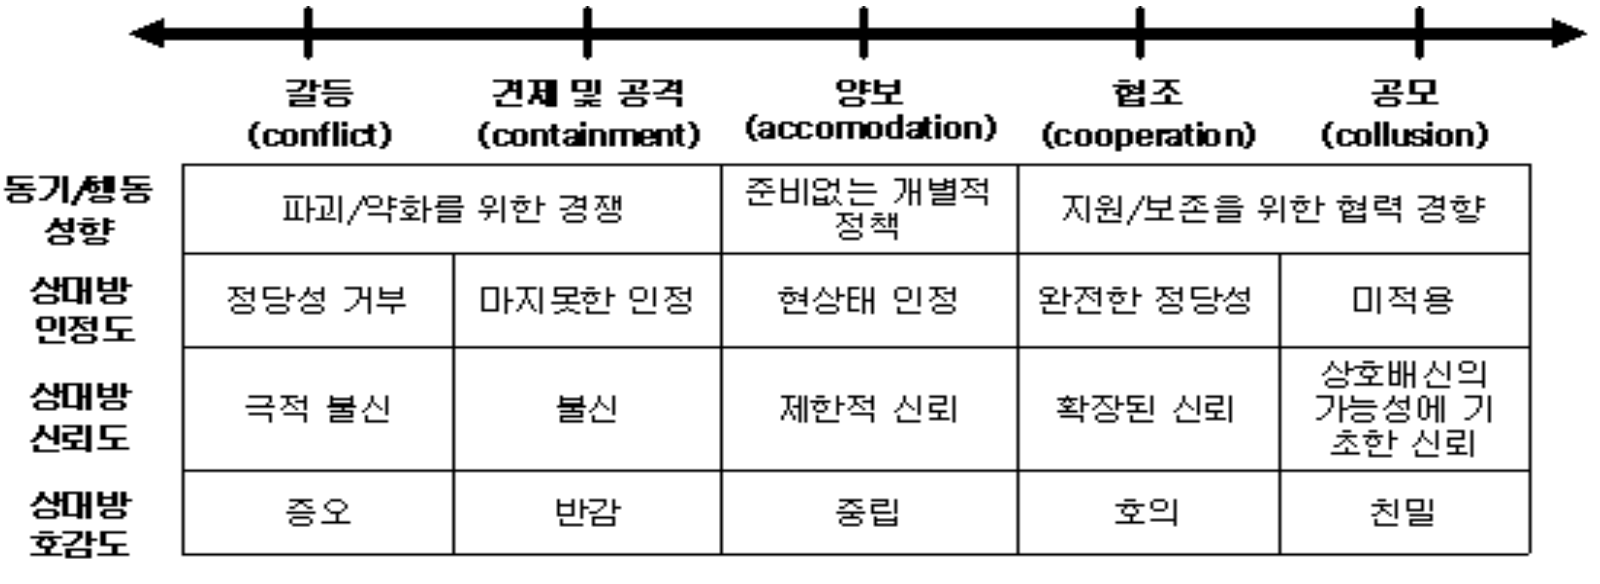
\includegraphics[width=.8\textwidth]{pic/노사협조개념도.png}
        \caption{노사협조의 개념}
    \end{figure}
    \begin{itemize}[<+->]
        \item 양 당사자의 사회적 상호작용의 관점에서 분석하여 보다 입체적으로 동기, 상대방 인정도, 신뢰도, 호감도의 여러 차원에서 구분
        \begin{itemize}[<+->]
            \item 갈등: 상대방을 파괴하고 약화시키기 위하여 노력. 상대방의 정당성을 거부하고 불신하며 증오
            \item 견제와 공격: 상대방의 정당성을 마지못해 인정하지만 여전히 불신하며 반감
            \item 양보: 상대방의 의견에 동의하여 자신의 주장을 수정하는 것으로 현상을 인정하고 상대방에 대하여 제한적으로 신뢰를 갖고 있으며 호감도는 중간 정도
            \item 협조: 호의를 가지고 상대방의 정당성을 완전히 인정하는 것에서 출발. 상대방의 목적을 달성할 수 있도록 노력하고, 서로의 조직을 강화시켜 주는 방식으로 작용
            \item 공모: 노사가 지나치게 친밀하여 서로의 본질에서 벗어난 행위를 하는 상태. 어용노조가 노조원의 권익에 피해는 주면서 사용자에게 협력하는 행위를 하는 경우
        \end{itemize}
    \end{itemize}
\end{frame}

\begin{frame}{노사협조에 대한 경제학적 이해}
    \begin{itemize}[<+->]
        \item 노사협조를 경제학적인 시각에서 `파이 굽기와 나누기' (baking and dividing pies)라는 비유를 활용하여 설명
        \begin{itemize}[<+->]
            \item 노사는 고용관계에서 야기되는 경제적 효용의 절대적 수준을 극대화하려는 공통의 이해관계를 가진고 있다고 주장
        \end{itemize}
        \item 노사 양측이 상대적 힘만을 발휘하여 절대효용을 극대화하려고 과도한 갈등을 초래할 경우 양 당사자 모두 얻는 것이 없게 됨 
        \begin{itemize}[<+->]
            \item 고용관계의 변합차원은 노사의 상대적 힘에 의한 함수가 아니라 노사의 조직적 힘을 결합한 함수를 구성하게 됨
        \end{itemize}
    \end{itemize}
\end{frame}
    
\section{경영참가}

\begin{frame}[allowframebreaks]{경영참가의 개념}
    \begin{itemize}[<+->]
        \item 경영참가: 노동자가 경영의 의사결정에 참가하는 것 (ILO의 정의)
        \begin{itemize}[<+->]
            \item 종래 경영자의 권한이라고 생각되어 온 이른바 경영권 또는 경영전권에 대하여 피고용인이나 노동조합이 그들의 이익을 지키고 또한 증진시킴을 목적으로 노사간에 공동으로 경영관리기능을 수행함
            \item 경영자와 함께 경영상의 권한과 책임 분담
        \end{itemize}
        \framebreak\relax
        \item 경영참가의 결과
        \begin{itemize}[<+->]
            \item 경영자가 갖는 의사결정상의 자유 제약
            \item 피고용인들의 자발성 신장 및 경영의 건전화 기대
            \item 피고용인도 무책임한 주장이나 경영자 권한의 통제 등을 자제
        \end{itemize}
        \item 산업민주주의를 목표로 함과 동시에 노사의 공동선을 목적으로 하는 장치이므로 쌍방의 이해관계가 충분히 반영되도록 노력하여야 함
    \end{itemize}
\end{frame}


\begin{frame}{경영참가제도의 유형}
    \begin{enumerate}[<+->]
        \item 자본참가
        \begin{itemize}[<+->]
            \item 자본의 출자자로서 기업경영에 참여 시키는 방식 
            \item 예: 우리사주제, 노동주 등
        \end{itemize}
        \item 성과참가
        \begin{itemize}[<+->]
            \item 피고용인 (노조)의 협력 대가로 경영성과 (업적·수익·이익)의 일부 분배 
            \item 예: 이익배분
        \end{itemize}
        \item 의사결정참가
        \begin{itemize}[<+->]
            \item 피고용인 (노조)이 경영의사결정에 참여하거나 경영기능에 대해 영향력을 행사 
            \item 예: QC, 노사협의회, 현장자율경영팀 등
        \end{itemize}
    \end{enumerate}
\end{frame}

\section{의사결정참가의 분류}

\begin{frame}[allowframebreaks]{참가근거}
    \begin{itemize}[<+->]
        \item 공식적 참가: 헌법, 각종 법규 및 시행령 등과 같은 법적 근거나, 노사간의 단체교섭에서 체결된 쌍방적 협약사항에 근거를 두거나, 경영자들의 일방에 의한 정책 및 제도로서 실시할 수 있는데 일정한 형식을 갖춘 기구를 통하여 참여하는 것을 의미
        \item 비공식적 참가: 경영자가 `그렇게 하는 것이 유익하기' 때문에 법이나 계약 등에 의거하지 않고 결정을 내리기 전에 하위자들의 조언이나 의견을 구하는 경우를 의미
        \begin{itemize}[<+->]
            \item 참여적 경영이 공식적인가 또는 비공식적인가 라는 문제는 본 프로그램을 설계한 사람의 가치관이나 참여적 경영을 실시함으로써 얻고자 하는 목적 및 기업의 상황 등에 따라서 달라질 수 있음
        \end{itemize}
        \item 일반적으로 유럽의 국가들은 공식적 참가를 사용하고 있는 반면에, 미국, 영국 등과 같은 앵글로 색슨계 국가들은 비공식적 참여를 실시
        \begin{itemize}[<+->]
            \item 유럽의 국가와 앵글로 색슨계 국가가 갖고 있는 역사적 발전과정, 사회적 특성, 법적 또는 정치적 체계, 및 노사관계시스템 등의 차이에 기인
        \end{itemize}
    \end{itemize}
\end{frame}

\begin{frame}{참가방식}
    \begin{itemize}[<+->]
        \item 직접적 참가: QC나 제안제도와 같이 작업장에서 개개 종업원이 의사결정과정에 직접 본인의 의견을 내놓는 것을 의미
        \item 간접적 참가: 노사협의회나 각종 위원회, 기타 의사결정기구에 종업원을 대표하는 노동조합이나 대표자를 통하여 이루어지는 참가형태
        \item 대체로 참여 수준이 높아질수록 간접적인 참가유형이 나타나고 있음
        \begin{itemize}[<+->]
            \item 사업장이나 그 이상의 참여에서는 대표자를 통한 간접적인 참가가 일반화되어 있기 때문
        \end{itemize}
    \end{itemize}
\end{frame}

\begin{frame}{참가강도}
    \begin{itemize}[<+->]
        \item 의사결정의 참가 강도를 세분화
        \begin{enumerate}[<+->]
            \item 의사결정에 관한 아무런 사전정보가 없는 경우
            \item 사전에 정보를 제공받는 경우
            \item 의사결정에 의견개진이 가능한 경우
            \item 노동자 의견이 의사결정에 고려되는 경우
            \item 의사결정에 대한 거부권을 가지는 경우
            \item 의사결정이 전적으로 구성원들에게 달려 있는 경우 등
        \end{enumerate}
    \end{itemize}
\end{frame}

\begin{frame}{참가의 내용}
    \begin{itemize}[<+->]
        \item 의사결정참가의 내용 차원은 학자간에 의견이 정리되지 못한 상황
        \item Locke \& Schweiger (1979)는 참여적 경영은 내용에 따라 4가지로 구분
        \begin{itemize}[<+->]
            \item 고용, 훈련 규율 및 성과평가 등과 같은 일상적인 인사관련 사항
            \item 과업할당, 직무설계 및 작업속도 등의 작업자체 사항
            \item 휴식, 작업시간, 작업의 배치 및 조명 등의 작업환경
            \item 해고, 이윤배분, 자본투자 및 전반적인 회사정책과 관련된 기업정책 등으로 구분
        \end{itemize}
        \item 일반적인 경향
        \begin{itemize}[<+->]
            \item 자발적·비공식적·직접적인 경우: 인사관련사항, 작업환경, 작업자체사항에 국한
            \item 강제적·공식적·간접적인 경우: 회사정책과 관련된 기업정책
        \end{itemize}
    \end{itemize}
\end{frame}

\begin{frame}{참가의 수준}
    \begin{itemize}[<+->]
        \item 전략적 수준 (strategic level)의 의사결정참가: 기업의 장기정책 혹은 전략의 의사결정과정에 종업원 혹은 종업원 대표가 참가하는 형태
        \item 기능적 수준 (functional level)의 의사결정참가: 단체협상이나 기업의 인사, 노무관리에 노동조합을 통하거나 각종 위원회를 통해서 참가하는 형태
        \item 작업장 수준 (workplace level)의 의사결정참가: 실제 작업장에서 발생하는 일상적인 활동이나 직무설계나 작업장 배치와 같은 종업원의 근무환경에 영향을 미치는 의사결정에 참가하는 형태
    \end{itemize}
\end{frame}

\begin{frame}[allowframebreaks]{참가 목적}
    \begin{itemize}[<+->]
        \item 경영참가를 보는 새로운 시각
        \begin{itemize}[<+->]
            \item 경영자 입장: 피고용인 또는 노동자 대표조직의 경영참가는 생산성 증대와 같은 조직 효율성을 제고하는 일반적 목적성을 가짐
            \item 경영참가를 보는 피고용인 입장: 산업민주주의의 실천이라는 오랜 전통의 노동운동 목표가 경영참여를 추구하는 가치 (형평성)의 기반이 됨
            \item 형평성은 효율성의 남용 (악용)으로부터 인간노동을 보호할 필요에서 비롯되고 또한 보다 높은 효율성을 달성하기 위해서는 인간노동을 공정하게 처리할 필요가 있음
        \end{itemize}
        \framebreak\relax
        \item 형평성 지향 경영참가: 인간으로서의 삶을 보장받기 위한 고용의 최저표준 설정, 산업민주주의 그리고 그러한 과정에의 적극적인 개입을 통해 절차 및 의사결정과정의 정당성을 확보하고자 하는 경영참여
        \begin{itemize}[<+->]
            \item 인사위원회, 징계나 해고와 관련된 참여, 복리후생적 노동조건의 개선, 인사고과 등에 관련된 참여 등
        \end{itemize}
        \item 효율성 지향 경영참가: 참여를 통해 노동자의 자율성과 창의성을 개발함으로써 이를 품질개선과 생산성 향상 등 조직성과의 향상에 기여할 수 있도록 하기 위해 설계, 추진되는 경영참여
        \begin{itemize}[<+->]
            \item 주로 사용자 주도적, 조직성과의 향상을 위한 다양한 혁신활동: QC, 제안활동, 문제해결팀 등
        \end{itemize}
    \end{itemize}
\end{frame}


%------------------------------------------------
\end{document}
%------------------------------------------------
